%%\documentclass[pdflatex,sn-nature]{sn-jnl}% Style for submissions to Nature Portfolio journals
%%\documentclass[pdflatex,sn-basic]{sn-jnl}% Basic Springer Nature Reference Style/Chemistry Reference Style
\documentclass[pdflatex,sn-mathphys-num]{sn-jnl}% Math and Physical Sciences Numbered Reference Style
%%\documentclass[pdflatex,sn-mathphys-ay]{sn-jnl}% Math and Physical Sciences Author Year Reference Style
%%\documentclass[pdflatex,sn-aps]{sn-jnl}% American Physical Society (APS) Reference Style
%%\documentclass[pdflatex,sn-vancouver-num]{sn-jnl}% Vancouver Numbered Reference Style
%%\documentclass[pdflatex,sn-vancouver-ay]{sn-jnl}% Vancouver Author Year Reference Style
%%\documentclass[pdflatex,sn-apa]{sn-jnl}% APA Reference Style
%%\documentclass[pdflatex,sn-chicago]{sn-jnl}% Chicago-based Humanities Reference Style

%%%% Standard Packages
%%<additional latex packages if required can be included here>

\usepackage{graphicx}%
\usepackage{multirow}%
\usepackage{amsmath,amssymb,amsfonts}%
\usepackage{amsthm}%
\usepackage{mathrsfs}%
\usepackage[title]{appendix}%
\usepackage{xcolor}%
\usepackage{textcomp}%
\usepackage{manyfoot}%
\usepackage{booktabs}%
\usepackage{algorithm}%
\usepackage{algorithmicx}%
\usepackage{algpseudocode}%
\usepackage{listings}%
\usepackage[english]{babel}
\usepackage{tikz}
\usetikzlibrary{shapes.geometric, arrows.meta, positioning}
%% as per the requirement new theorem styles can be included as shown below
\theoremstyle{thmstyleone}%
\newtheorem{theorem}{Theorem}%  meant for continuous numbers
%%\newtheorem{theorem}{Theorem}[section]% meant for sectionwise numbers
%% optional argument [theorem] produces theorem numbering sequence instead of independent numbers for Proposition
\newtheorem{proposition}[theorem]{Proposition}% 
%%\newtheorem{proposition}{Proposition}% to get separate numbers for theorem and proposition etc.

\theoremstyle{thmstyletwo}%
\newtheorem{example}{Example}%
\newtheorem{remark}{Remark}%

\theoremstyle{thmstylethree}%
\newtheorem{definition}{Definition}%

\raggedbottom
%%\unnumbered% uncomment this for unnumbered level heads

\begin{document}

\title[Article Title]{Report}

\author{\fnm{} \sur{}}

\maketitle

\section{Abstract}
%sam did this
Strong gravitational lensing of gravitational waves (GWs) is an expected consequence of the propagation of compact binary signals through an inhomogeneous universe, and a small but non-zero fraction of events detected by ground based observatories should be multiply imaged by intervening galaxies or clusters \cite{2}\cite{6}\cite{18}\cite{19}.
Recent forecasts indicate that the first confident strongly lensed GW detection could occur during the fifth LIGO-Virgo-KAGRA observing run (O5)\cite{19}, while searches incorporating 01-O4a events forecast a substantial probability of reaching at least $3\sigma$ significance in O5\cite{20}.
At the same time, simulations based on the Hubble Space Telescope (HST) quality imaging show that resolved electromagnetic (EM) strong lensing data can constrain the lens potential at the sub-percent level in a favourable GW+EM systems \cite{21}.
Motivated by these results, this work develops a Bayesian framework in which a catalogued lens with resolved strong lensing information ($H_1$) is used to increase the confidence of a candidate lensed GW pair.
The central forecast to be tested is that targeted HST follow-up can, for favourable $H_1$ systems, sharpen the lens prediction sufficiently to raise the strong lensing detection confidence toward $5\sigma$. We derive the full $H_1$ evidence, (insert natalie) and (insert harry). The remaining hypotheses describe a catalogued lens without resolved images ($H_2$), an uncatalogued lens ($H_3)$, and two independent unlensed BBHs ($H_U$).\\
Keywords: gravitational waves; gravitational lensing: strong; Bayesian inference; electromagnetic catalogues; binary black holes; multi-messenger astronomy.

\section{Introduction}
%sam did this
Gravitational waves propagate along null geodiscs and are therefore subject to gravitatioanl lensing in the sam manner as electromagnetic radiation in the geometric optics limit \cite{1}\cite{2}. 
For galaxy scale lenses, a single compact binary coalescence can produce multiple detectable images separated by minutes to months, depending on the lens potential and source geometry. 
To leasing order, the images share the same intrinsic binary paramters while differing in arrival time, amplitude through the lensing magnification, and an image type dependent phase contribution \cite{3}\cite{4}\cite{5}\cite{6}. 
This repeated signal structure motivates searches for pairs or multiples of GW events that are mutually consistent under a common source hypothesis.\\
\\The central statistical difficulty is that an unlensed population can also produce event pairs with overlapping posterior distibutions.
A robust lensing claim must therefore compare a common source moel against a model in which the detections arise from independent binaries.
Bayesian model selection provides a natural framework because it combines likelihood agreement, prior information, population expectations and parameter space volume into a single evidence ratio \cite{7}\cite{8}\cite{9}.
Early work proposed posterior overlap statistics for lensed GW indentification \cite{3}, while subsequent analyses incorporated lensing time-delay distributions, astrophysical populations, selections effects and full join parameter estimation \cite{7}\cite{8}\cite{9}\cite{10}.
Searches of LIGO-Virgo-KAGRA data have so far found no compelling population level evidence for strong lensing, reinforcing the need for careful prior odds and follow up tests \cite{12}\cite{13}\cite{14}.\\
\\A major source source of additional information is the electromagnetic foreground.
A galaxy or cluster capable of producing strong lensing may be visable in wide field imaging or spectroscopic catalogues even when the binary black hole (BBH) source itself has no EM counterpart.
The EM data may range from a simple galaxy detection with photometry and redshift information to a resolved strong lensing system with arcs or multiple images of an unrelated background source.
Such data can constrain the lens mass distribution, position, redshift and velocity scale, and therefore predict distributions for the same lensing observables, such as relative time delay and magnification ratio, that are inferred from the GW pair.
Recent work on lens reconstruction and catalogue informed priors further demonstrates that EM information can break degeneracies that remain in GW only analyses and can materially alter lensing odds \cite{15}\cite{16}\cite{17}.

\section{Methodology}
\subsection{Simulated GW events and Bayesian Parameter Estimation}
(Consult Ankur)

\subsection{Population Reconstruction}
% Natalie's part
importance, posterior samples, non-parametric, (H)DPGMM, FIGARO, uncertainties (blue region), limitations (not intrinsic)\\
The population distribution of binary black hole (BBH) parameters is crucial for determining whether two similar gravitational wave (GW) signals come from the same source, or belong to two pairs of BBH with very similar properties.\\
Intuitively, ...\\
Mathematically, ...\\
Population reconstruction on a simulated distribution of BBHs is performed using FIGARO, which uses a non-parametric approach to model probability densities using a Dirlchlet Process Gaussian Mixture Model. (More detailed descriptions). 
Many draws, uncertainties; does not reflect intrinsic population\\
Used to compute prior odds, Bayes factor, ...

\subsection{Prior Odds Estimation}
% Natalie's part
definition, formula (cite Otto's paper), how each component is calculated (ler)

\section{Bayesian hypothesis space}
%sams part
Consider two GW detections, $d_{GW}={d_{GW,1},d_{GW,2}}$, together with EM observations dEM drawin from a catalogue of potential foreground lenses. 
We divide the lensing interpretation into three mutually exclusive observational cases and compare their union with an unlensed alternative.
\begin{table}[h]
\centering
\caption{Mutually exclusive hypotheses used in the joint GW-EM model comparison}
\label{}
\begin{tabular}{|p{2cm}|p{3cm}|p{4cm}|}
\hline
Hypothesis & GW interpretation & EM/catalogue information \\ \hline
$H_1$       & Two detections are lensed images of the same BBH.        & The repsonsible lens is catalogues and resolved strong-lensing EM information constrains a detailed lens model.         \\ \hline
$H_2$       & Two detections are lensed images of the same BBH.        & The responsible lens is catalogues, but no resolved strong-lensing image configuration is available; EM data constrain galaxy properties.        \\ \hline
$H_3$       & Two detections are lensed images of the same BBH.        & The responsible foreground lens is absent from the catalogue.              \\ \hline
$H_U$       & The detections arise from two independent unlensed BBHs.         & Any galaxy in the search region is treated as an unrelated field object, conditional on the search selection.              \\ \hline  
\end{tabular}
\end{table}
\begin{equation}
H_L = H_1 \cup H_2 \cup H_3
\end{equation}
with $H_1$, $H_2$ and $H_3$ mutually exclusive within the assumed search space. 
The posterior probability of the total lensed hypothesis is therefore
\begin{equation}
p(H_L|d) = p(H_1|d) + p(H_2|d) + p(H_3|d)
\end{equation}
where $d={d_{GW},d_{EM}}$. For each model $H_i$, Bayes' theorem gives
\begin{equation}
p(H_i|d) = Z_i \frac{p(H_i)}{p(d)}, Z_i \equiv p(d|H_i).
\end{equation}
The posterior odds of lensing relative to the unlsened hypothesis are consequently
\begin{equation}
\frac{p(H_L|d)}{p(H_U|d)} = \frac{[Z_1p(H_1) + Z_2p(H_2) + Z_3p(H_3)]}{Z_Up(H_U)}
\end{equation}
Equation (above) makes the role of the hypothesis prior explicit. 
The Bayes factor quantifies how the data update the relative support for the models, while the prior odds encode the expected rarity of strong lensing and the probability that a responsible lens belongs to each catalogue class. 
This distinction is important because prior odds and search selection can change substantially as the GW catalogue grows [7,9,14].

\section{Parameterisation and Conditional Structure}
\subsection{Binary Black Hole Source Parameters}
Let $\theta_{BBH}$ denote the physical parameters of the compact binary source.
A representative set is
\begin{equation}
\theta_{BBH}=\{m_1,m_2,\chi_1,\chi_2,z_s,\Omega_s,\iota,\phi_{pol},...\}.
\end{equation}
The exact waveform parameterisation mat instead use detector frame masses, luminosity distance and spin coordinates.
Under any lensed hypothesis, the intrinsic source parameters are shared by the images, whereas under $H_U$ the two detections have independent parameter sets $\theta_{BBH,1}$ and $\theta_{BBH,2}$.
Apparent luminosity distances are image dependent because magnification rescales the observed strain amplitude.

\subsection{Lens and Source Plane Parameters}
The lens is described by a model dependent parameter vector
\begin{equation}
\theta_{lens}={z_l,\sigma_v,q,\phi_l,\Omega_l,\gamma_{ext},\phi_{ext},...}
\end{equation}
where $z_l$ is the lens redshift, $\sigma_v$ s velocity dispersion or equivalent madd scale parameter, $q$ the projected axis ratio, $\phi_l$ the lens orientation, $\Omega_l$ the lens position, and $\gamma_{ext}$ and $\phi_{ext}$ describe external shear.
The source position $\beta$ relative to the caustic must also be included.

\subsection{Image Level Lensing Observables}
The GW pair constrains a lower dimensional set of relations between the images.
We denote these by
\begin{equation}
\psi_{GW}={\Delta t, \mu_r, \Delta n, \Omega, ...}
\end{equation}
where $\Delta t$ is the relative arrive time delay, $\mu_r$ is a relative magnification ratio, $\Delta n$ denotes the relative mMorse index, and $\Omega$ represents common sky localisation.
These quantities are not independent free parameters in a physical lens model; they are generated by the lens equation and Fermat potenital,
\begin{equation}
\psi=f(\theta_{lens},z_s,\beta;cosmology).
\end{equation}
This mapping is the bridge between the GW and EM analyses: the GW data constrain $\psi$ directly or semi-directly, while EM observations constrain $\theta_{lens}$ and thereby induce a predictive distribution for $\psi$.

\subsection{Electromagnetic Nuisance Parameters}
EM observations require nuisance parameters $\nu_{EM}$ describing measurement and modelling uncertainties.
Depending on the catalogue and imaging data, $\nu_{EM}$ may include the point spread function, photometruc calibration, specral energy distribution parameters, stellar mass to light ratio, background subtraction, photometric redshift calibration and other instrument or population level terms.
These parameter should be maginalised rather than fixed when their uncertainty is non negligible, beause overly narrow EM constraints can artificially increase the GW-EM consistency factor.

\section{Unlensed Hypothesis}
%sam
Under $H_U$ the detections correspond to two independent BBH mergers.
The GW evidence is
\begin{equation}
Z_{GW,U} = \int p(d_{GW,1}|\theta_{BBH,1},H_U) p(d_{GW,2}|\theta_{BBH,2},H_U) \pi_U(\theta_{BBH,1},\theta_{BBH,2})d\theta_{BBH,1}d\theta_{BBH,2}
\end{equation}
The EM observations must not be allowed to depend pn whether the GW pair happens to be unlensed.
We therefore introduce an EM field model, $H_{EM,field}$, that describes unrelated foreground galaxies under the same catalogue/search selection.
When the GW and EM data are conditionally independent under $H_U$,
\begin{equation}
H_U \equiv H_{GW,U} \cap H_{EM,field}
\end{equation}
\begin{equation}
Z_U = Z_{GW,U} Z_{EM,field}, Z_{EM,field} = p(d_{EM}|H_{EM,field})
\end{equation}
This term is essential whenever the lensed hypotheses recieve evidence from the existence or properties of a catalogue galaxy.
Omitting the corresponding field galaxy probability from $H_U$ would systematically favour catalogues lens hypotheses simply because a galaxy was searched for and found.

\section{$H_1$: catalogued lens wit resolved strong lensing information}
%sam
\subsection{Resolved EM data and parameter set}
%sam
Under $H_1$, the two GW detections are strongly lensed images of the same BBH and the responsible foreground lens is present in the EM catalogue with resolved strong lensing information.
(not sure about this but had a thought) The resolved EM source need not be the BBH counterpart; it provides an independednt probe of the same foreground gravitational potential.
The EM data may therefore be separated schematically into measurements of the lens galaxy and measurements of the resolved strong lensing configuration.
\begin{equation}
d_{EM,c} = \{d_{gal,c},d_{SL,c}\}
\end{equation}
Here $d_{gal,c}$ may contain quantities such as lens position, redshift, photometry, and velocity dispersion, while $d_{SL,c}$ may contain resolved image positions, arc, an Einstein ring or pixel level surface brightness data.
The exact observables depend on the survey and lens modelling procedure.\\
\\
The parameter vector is
\begin{equation}
\Theta_1 = \{\theta_{BBH},\theta_{lens},\beta_{GW},\theta_{EMsrc},\beta_{EMsrc},\nu_{EM}\}
\end{equation}
The parameters $\Theta_{BBH}$ describe the common BBH source, $\theta_{lens}$ describes the foreground mass model, and $\beta_{GW}$ is the BBH source plane position.
The parameters $\theta_{EMsrc}$ and $\beta_{EMsrc}$ describe the independently lansed background EM source, while $\nu_{EM}$ contains observational nuisance parameters such as the point spread function, calibration, sky background and noise model.
The central coupling is that the same $\theta_{lens}$ appears in both the GW and EM likelihoods.\\
\\Conditional on $\Theta_1$, the joint data model is
\begin{equation}
p(d_{GW},d_{EM,c}|\Theta_1,H_1) = p(d_{GW}|\theta_{BBH},\theta_{lens},\beta_{GW},H_1)p(d_{EM,c}|\theta_{lens},\theta_{EMsrc},\beta_{EMsrc},\nu_{EM},H_1)
\end{equation}

\subsection{Full joint evidence and prior}
%sam
For a catalogue candidate c, the primary model selection quantity is the full joint evidence
\begin{equation}
Z_{1,c} = \int p(d_{GW}|\theta_{BBH},\theta_{lens},\beta_{GW},H_1)p(d_{EM,c}|\theta_{lens},\theta_{EMsrc},\beta_{EMsrc},\nu_{EM},H_1)\pi_1(\Theta_1)d\Theta_1
\end{equation}
A useful schematic prior factorisation is
\begin{equation}
\pi_1(\Theta_1)=\pi_{BBH}\pi_{lens}\pi_{\beta,GW}\pi_{\nu,EM}S_1
\end{equation}
where $S_1$ denotes the required GW detection, catalogue and resolved lens selection conditioning.
This factorisation is schematic: correlations implied by a population model or a particular lens modelling analysis should be retained rather than forced into independent factors.

\section{Result}
\subsection{Reconstructed Population}
% Natalie's part
(Will replace the following with the new plot when script finishes running)
\begin{figure}[ht]
    \centering
    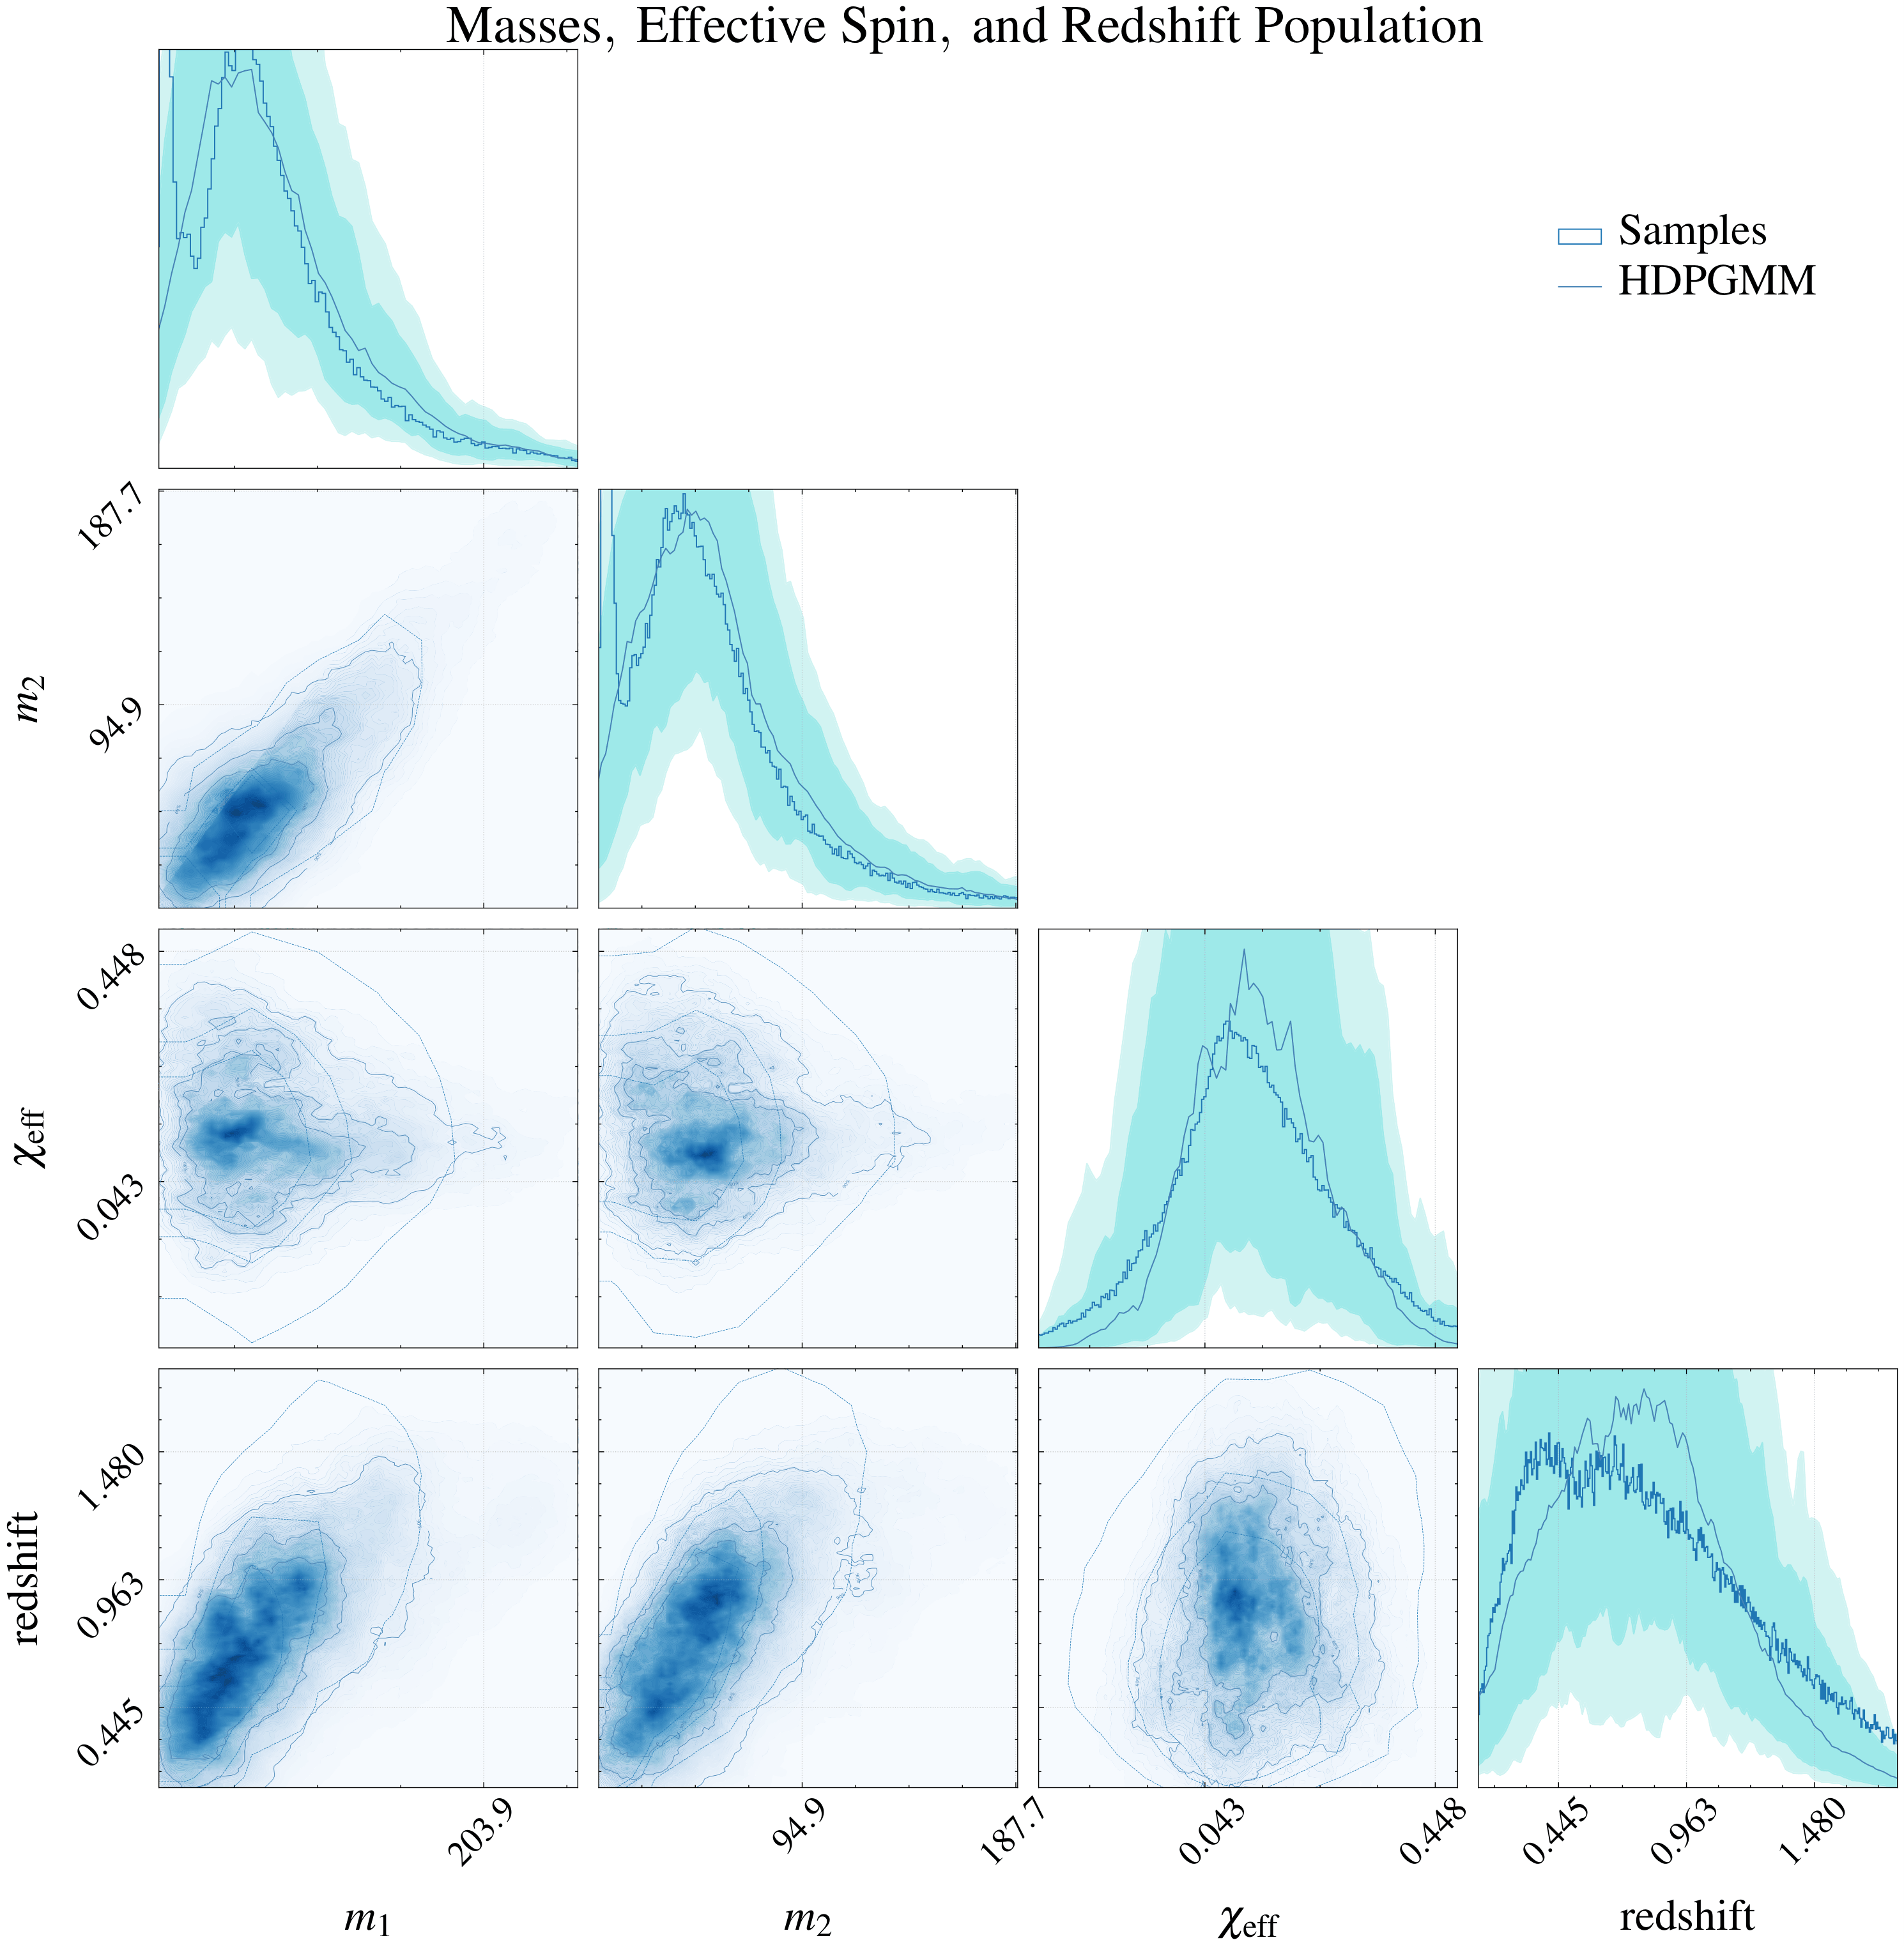
\includegraphics[width=0.8\textwidth]{figures/reconstructed_population.png}
    \caption{Corner plot of the reconstructed binary black hole population in component masses ($m_1, m_2$), effective spin ($\chi_\text{eff}$), and redshift using the hierarchical DPGMM implementation in FIGARO. The diagonal panels show the one-dimensional marginal distributions, while the off-diagonal panels show the corresponding two-dimensional joint distributions.}
    \label{fig:reconstructed_population}
\end{figure}

\subsection{Prior Odds}
% Natalie's part
rates, rate ratio, prior odds.


\section{Conclusion}

\bibliography{references}% common bib file

\section{Appendix}

\end{document}
